\documentclass[colorlinks=true,pdfstartview=FitV,linkcolor=blue, citecolor=red,urlcolor=magenta]{ligodoc}

\usepackage{graphicx}
\usepackage{amssymb}
\usepackage{amsmath}
\usepackage{longtable}
\usepackage{rotating}
\usepackage[usenames,dvipsnames]{color}
\usepackage{fancyhdr}
\usepackage{subfigure}
\usepackage{hyperref}
\usepackage{hhline}
\usepackage{wrapfig}
\usepackage{lineno} % adding line number
% \linenumbers


\renewcommand{\tan}{\mathop{\rm tg}\nolimits}
\newcommand{\bra}[1]{\langle#1|}
\newcommand{\ket}[1]{|#1\rangle}
\newcommand{\bracket}[2]{\langle#1|#2\rangle}
\newcommand{\mean}[1]{\langle#1\rangle}
\newcommand{\means}[1]{\langle#1\rangle_{sym}}
\newcommand{\Tr}[1]{\textbf{Tr}\{#1\}}
\newcommand{\dt}[1]{\frac{\partial #1}{\partial t}}
\newcommand{\I}[2]{\int\limits_{#1}^{#2}\,}
\newcommand{\note}[1]{\textcolor{red}{#1}}


\ligodccnumber{T}{12}{00383}{}{v1}
% \ligodistribution{AIC, ISC}
\graphicspath{{images/}}

\bibliographystyle{unsrt}
\title{Adaptive Quantum Measurements in Future Gravitational-wave Detectors}

\author{Mikhail Korobko, Haixing Miao, and Yanbei Chen}

\begin{document}
% \section{Notation}
$\mathbf{y}$ is $N\times1$ vector
$x$ is $p\times1$ vector
$\mathbb{D}$ is $N\times p$ matrix
$\mathbb{N}$ is $N\times N$ matrix
$\mathbb{L}$ is $p\times N$ matrix
\section{Introduction and motivation}
Contemporary so-called second-generation gravitational-wave detectors, such as Advanced LIGO \cite{AdvLIGOsite, Harry2010},
 Advanced VIRGO \cite{AdvVIRGOsite}, and LCGT \cite{LCGTsite}, which are under construction now, will be quantum noise limited.
Two quantum noises will limit the sensitivity: the phase fluctuations of the light inside the interferometer (shot noise) at high gravitational wave frequencies
and the random force created by the amplitude fluctuations of the light (radiation-pressure noise) at low frequencies.
For balanced detector the best sensitivity point - where these two noise sources become equal -
 is known as the Standard Quantum Limit (SQL) \cite{92BookBrKh}.
In the linear position meter (the gravitational-wave interferometer is special case of it)
the shot noise corresponds to the measurement noise and radiation pressure noise - to the back-action noise.
 Spectral densities of these noises obey the Heisenberg uncertainty relation \cite{92BookBrKh}.
The SQL is not an absolute limit for measurement precision: there are few methods of overcoming it in gravitational-wave detectors. The most well-known examples are
Quantum Non-Demolition (QND) measurements and Back-Action Evading (BAE) measurements (see, {\it e.g.},
 \cite{90a1BrKh, Buonanno2001m, 01a2Kh, 02a1KiLeMaThVy}). The first method supposes using the Hamiltonian
 of interaction the test body and measurement device,
which commutes with operator of measured quantity \cite{77a1eBrKhVo, 90a1BrKh, 96a1BrKh, 92BookBrKh}. The second method uses the
correlation between the measurement noise and the back-action noise.\cite{Unruh1982, 87a1eKh, JaekelReynaud1990, Pace1993, 96a2eVyMa, 02a1KiLeMaThVy}

In planned third generation detectors,like Einstein Telescope gravitational-wave detector \cite{Sathyaprakash2011} using these methods is supposed,
 that should provide sensitivity better than the SQL. However, both of them require sufficient
 modification of existing experimental schemes and have some technical difficulties (for example, variational-readout scheme is sensitive to optical losses [?]).

In our work we want to investigate the other approach - adaptive linear measurements. The idea is to change
 the parameters of the scheme depending on the results of previous measurements. Our aim was to create the effective algorithm for quantum adaptive measurements,
 check whether we can overcome SQL and compare it to the existing methods.



\section{Conception of adaptive measurements}\label{sec:concept}
\subsection{Estimation of parameters}
In wide class of the experiments the main goal can be described as follows: we have ``black box'' with some output that we can measure, and the idea is to get information about parameters of this ``black box'' using only this output signal. The problem is that we have some noises acting on our system. The procedure of estimation of the parameters from noisy signal is called filtering. To specify the problem, let's take a look of Fig.\ref{pic:stfilt},where we have some dynamical system with output signal $x(t)$ (this value can be a vector). We proceed measurements and have some data $y(t)$; then use filter and get some estimated value $\tilde{x}(t)$. 
The choice of filtering procedure depends on the particular problem. Most common filters minimize error or mean square error, but there are plenty of other.  
We call optimal the filter that achieves best estimation. 
% This approach is part of the control and estimation theory \cite{Slotine1991} and has lot of applications, particularly it can be used in quantum measurements \cite{Wiseman2011a}.
\subsection{Adaptive filtering}

\begin{figure}
\vspace{-5ex}
\begin{minipage}{0.6\linewidth}
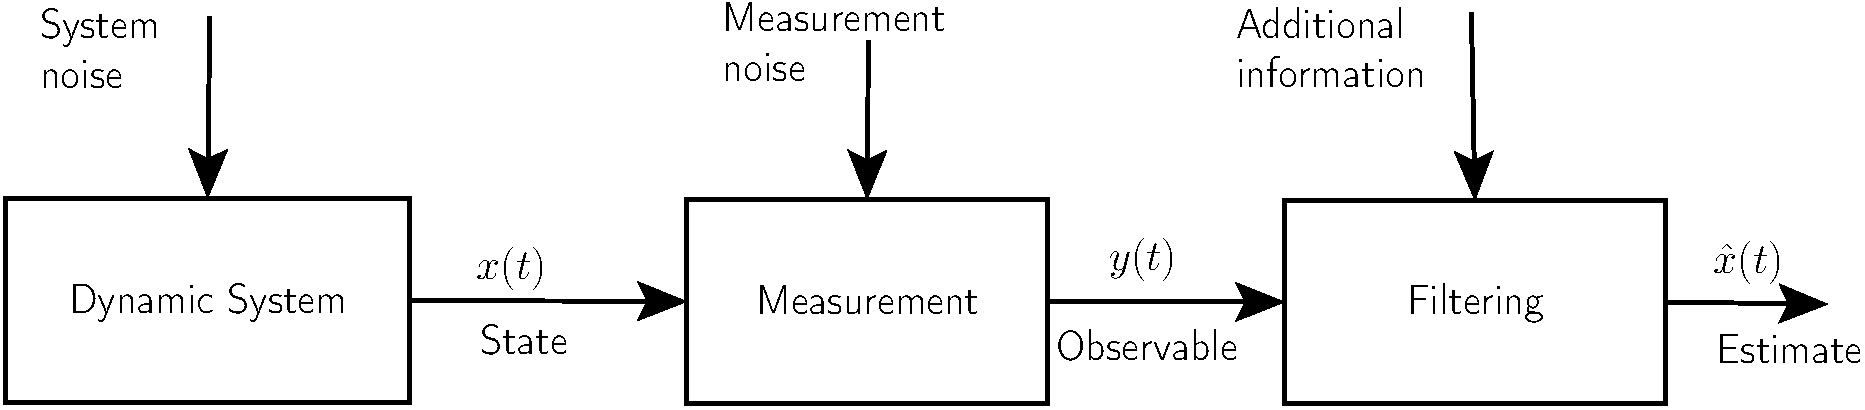
\includegraphics[width=1\linewidth]{meas_dia.pdf}
\caption{Classical filtering problem}
\label{pic:stfilt}
\end{minipage}
\hfill
\begin{minipage}[h]{0.4\linewidth}
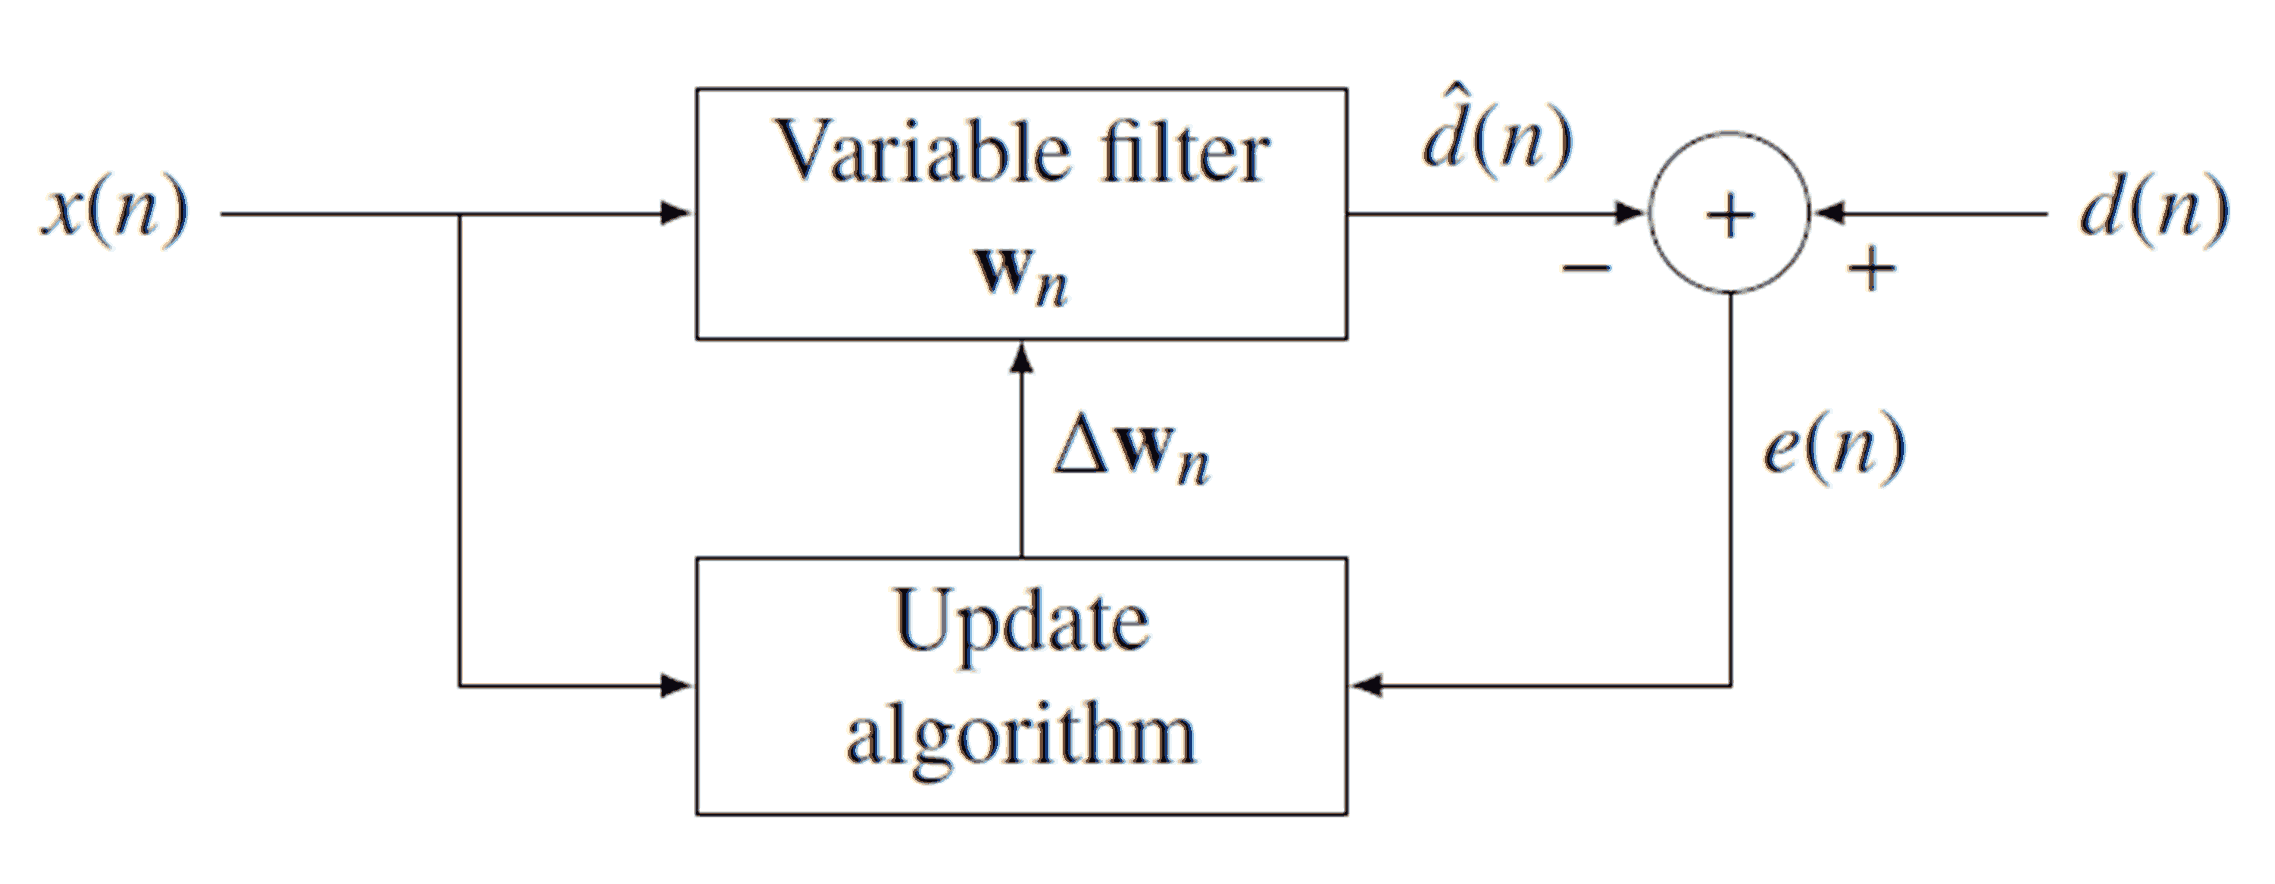
\includegraphics[width=1\textwidth]{AdaptiveFilter_C.png}
\caption{\footnotesize Block-scheme of the adaptive filter. Here $x(n)$ is signal, $\tilde{d}(n)$ is estimation of desired signal $d(n)$ and $e(n)$ is error.}
\label{pic:ad1}
\end{minipage}
\end{figure}

One of the way of solving filtering problem is so-called adaptive filtering. Adaptive filter adjusts its filtering function using error signal in order to achieve optimal filtering \cite{Farhang-Boroujeny1998,Sastry1989,Haykin2003,Drumright1998,Nationale1991,Huzmezan2002}.
Classic adaptive filter has quite simple scheme: as illustrated in Fig. \ref{pic:ad1}, we estimate the output signal in order to reach desired value. On the each step we use an error between estimated signal an desired to change the adaptive filter.
\\
But in the quantum case there are significant differences: the most important is presence of uncertainty principle, so we can not measure, for example, two different optical quadratures (or position and momentum) with any precision. Also we can not disturb the signal from system before measurement, otherwise we loose information about the state of the system.
That is why we have to modify existing schemes for quantum case.
We propose the following scheme for quantum case as shown in Fig. \ref{pic:quantad}\\

The procedure of such filtering is the following:
\begin{enumerate}
 \item $x(t)$ is a signal from the system, we measure it and get $\tilde{y}(t)$, then filter it in order to get estemation $\tilde{x}(t)$
 \item We use this estimation as initial state for the second stage. During this stage our initial state evolves and then we measure it and get second estimation $\tilde{\tilde{y}}(t+\varDelta t)$
 \item We make measurements at the time $t+\varDelta t$ and get approximation $\tilde{y}(t+\varDelta t)$
 \item Calculating error $\varepsilon(t+\varDelta t) = \tilde{\tilde{y}}(t+\varDelta t) - \tilde{y}(t+\varDelta t)$  and using errors in previous moments we can predict the optimal filter at time $t+2 \varDelta t$
 \item Now we can change this filter according to our prediction
\end{enumerate}

So, at each step of our measurement procedure we do the following stages of optimal quantum measurements: preparation(``create'' the state $\tilde{x}$)\cite{Rehbein2009m}, evolution(wait some small time $\varDelta t$) and verification(the second approximation and optimization of the filter)\cite{Miao}

\begin{figure}[!]
\begin{center}
 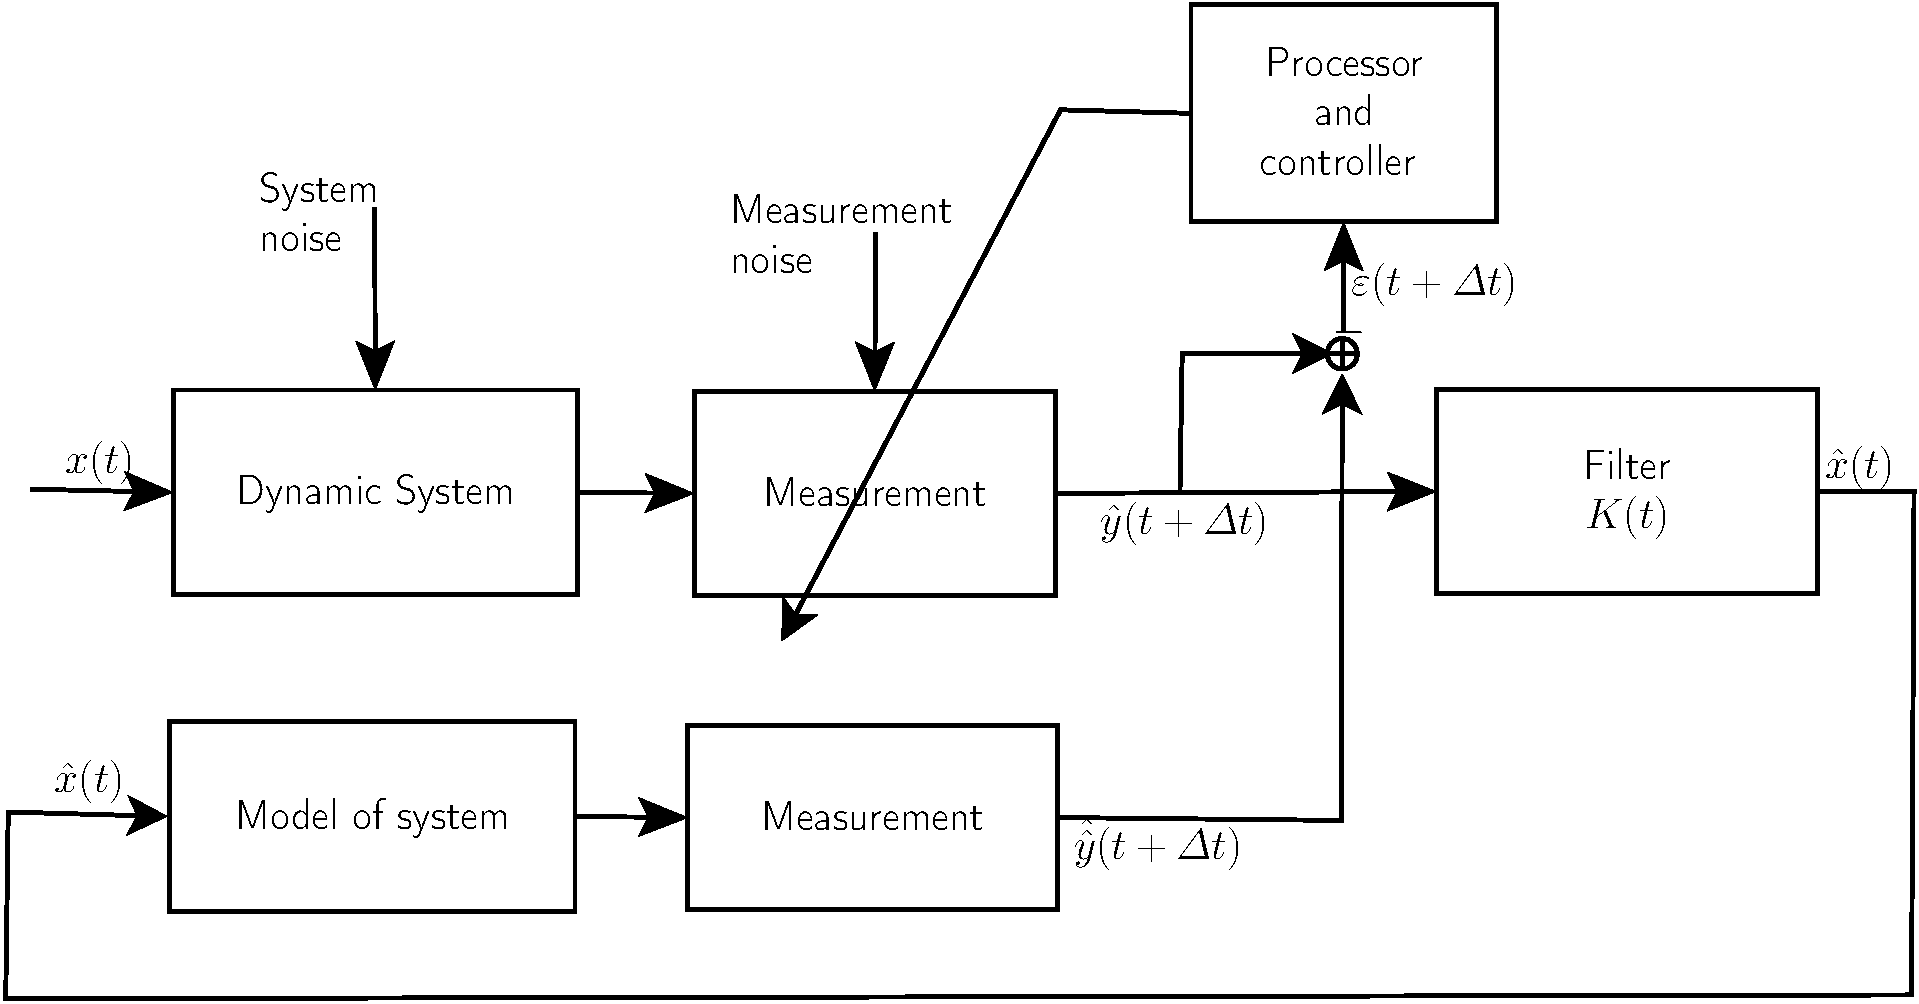
\includegraphics[width=1\linewidth]{adapt_1.pdf}
 \caption{Adaptive filter for quantum measurements}
\label{pic:quantad}
\end{center}
\end{figure}
In spite of the fact that classical case and quantum one have lots of differences, both of them can be described by similar equations,well known from control theory.
% \subsection{Application}
% This idea can be easily applied to our particular case of GW detection. We consider the usual interferometer with homodyne detection, but we change the homodyne angle in that way to minimize the cost function for next measurement. Such scheme would be adaptive and probably can help us to deal with some specific tasks. We shall discuss it later.

\begin{figure}
\begin{minipage}[b]{0.6\linewidth}
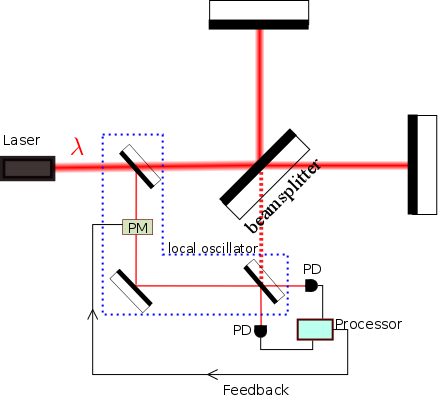
\includegraphics[width=1\textwidth]{ad_m.png}
\caption{Scheme of adative measurements for interferometer}
\end{minipage}
\hspace{0.1\linewidth}
\begin{minipage}[b]{0.3\linewidth}
 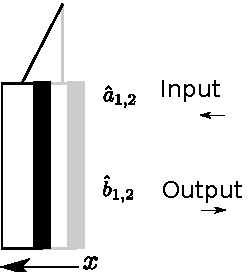
\includegraphics[width=1.0\textwidth]{system}
 \caption{Model of the system}
 \label{pic:sys}
\end{minipage}

\end{figure}
\subsection{Previous researches}
Due to the clearness of the idea, adaptive measurements are extremely popular in classical experiments. There are some fields of application, such as noise cancelling, seismic data processing,beamforming, \textit{etc.} \cite{Farhang-Boroujeny1998}
Currently the quantum adaptive control is a fast developing field \cite{Wiseman2011a,Ahn2008}, and some of the works were devoted to the adaptive filtering.
The main idea of adaptive quantum measurement was proposed almost at the same time at different scientific groups \cite{Wiseman1997,Braginsky1993}.The significant contribution was made by Wiseman and Berry is series of papers on adaptive measurements of phase of the light \cite{Berry2008,Berry2001,Berry2002,Measurements1995m}
By the moment there are a few works on the adaptive measurements in GW detectors \cite{Hentschel2010,Dhurandhar2008}.

In my work I investigate some new ideas: firstly I consider a new scheme for adaptive measurements and general method for solving such tasks, secondly, I consider the case of opto-mechanical system (not just optical, as in previous works), and thirdly, I provide some real estimation for LIGO experiment in order to make a decision if such an approach could be feasible to realize.

\section{Adaptive filtering: theory}\label{sec:th}
\subsection{System}

\begin{figure}
\center{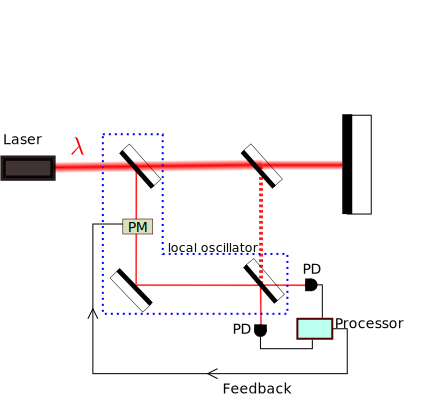
\includegraphics[width=0.5\textwidth]{adaptive_scheme}}
\caption{Optomechanical system}
\label{scheme}
\end{figure}

We consider simple optomechanical system of oscillator and homodyne detector (see Fig.\ref{scheme})\\
The oscillator can be described with following equation of motion:
\begin{equation}
\begin{cases}
 \dot{\hat{x}}(t) &= \frac{\hat{p}(t)}{m},\\
 \dot{\hat{p}}(t) &= -2\gamma \hat{p}(t) - m\omega_m^2 \hat{x}(t) + \alpha \hat{a}_1(t),
\end{cases}
\end{equation}
where $\alpha \hat{a}_1(t)$ corresponds to back-action noise, $\alpha$ is coupling constant between the oscillator and optical field.
So, for the ingoing optical fields $\hat{a}_{1,2}$ and outgoing $\hat{b}_{1,2}$ (see Fig. \ref{pic:sys}) we get following input-output relations:
\begin{equation}
\begin{cases}
 \hat{b}_1(t) &= \hat{a}_1(t),\\
 \hat{b}_2(t) &= \hat{a}_2(t) + \frac{\alpha}{\hbar}\hat{x}(t)\label{b2_general}.
\end{cases}
\end{equation}

Here we introduced ingoing and outgoing optical fiels. In the paraxial and narrowband approximation they are related with strength of electrical field as:
\begin{equation}
 \hat{E}(t) = \sqrt{\frac{4\pi \hbar\omega_0}{\mathcal{S} c}} \bigl[\bigl(\bar{a}+\hat{a}_1(t)\bigr)\cos\omega_0t + \hat{a}_2(t)\sin\omega_0t\bigr],
\end{equation}
where $\bar{a}$ is classical amplitude and $\mathcal{S}$ is effective cross-section area of the laser beam. A similar equation holds for the outgoing fields $\hat{b}_{1,2}$.
Other important fact is commutators of the field operators:
\begin{equation}
 \bigl[\hat{a}_1(t),\hat{a}_2(t')\bigl] = \bigl[\hat{b}_1(t),\hat{b}_2(t')\bigl] = i \delta(t-t').
\end{equation}
Then we can write the correlation functions:
\begin{equation}
 \means{\hat{a}_i(t) \hat{a}_j(t')} = \frac{1}{2}\delta_{ij}\delta(t-t'), \quad i,j=1,2.
\end{equation}

In Eq.\ref{b2_general} we inroduced $\hat{x}(t)$ as general solution for harmonic oscillator: 
\begin{equation}\label{sol_osc}
  \hat{x} = \hat{x}(0) \cos \omega_m t+ \frac{\hat{p}(0)}{m \omega_m} \sin \omega_m t + \int\limits_0^\infty \, dt' \, G(t-t')\Theta(t-t')(F(t)+\alpha \hat{a}_1(t')),
\end{equation}
where $F(t)$ is external force acting on the oscillator and we define Green's function of the oscillator as $G(t)=\frac{\sin \omega_m t}{m \omega_m}$ and $\Theta(t)$ is Heaviside function.
In general case the shape of the external force is unknown.

For detection a signal we use homodyne detector with local oscillator's phase changing in time. The output optical field
\begin{equation}
 \hat{B}_{out}(t) = \hat{b}_1(t)\cos \omega_0 t +  \hat{b}_2(t) \sin \omega_0 t
\end{equation}
mixes with local oscillator light
\begin{equation}
 L(t)=L_c(t)\cos \omega_0 t + L_s (t) \sin \omega_0 t = L_0 \cos (\omega_0 t + \zeta(t)).
\end{equation}
The resulting photocurrent is
\begin{multline}
 i(t) = i_1(t)-i_2(t) = \frac{1}{2}\bigl( \overline{(L(t)+\hat{B}_{out}(t))^2}- \overline{(L(t)-\hat{B}_{out}(t))^2}\bigr) = 2 \overline{L(t)\hat{B}_{out}(t)} =\\
=L_0 \hat{b}_1(t)\cos \zeta(t) +  L_0 \hat{b}_2(t) \sin \zeta(t).
\end{multline}

So, we can rewrite the output as:
\begin{equation}\label{gen_y}
 \hat{y}(t) = \hat{b}_1(t)\cos \zeta(t) +  \hat{b}_2(t) \sin \zeta(t),
\end{equation}
and our main task would be search of the optimal homodyne angle $\zeta(t)$ for any moment of time. We can do this using adaptive measurements.

\subsection{Adaptive measurements: general approach}
In our work we consider simple case of impulse force with unknown amplitude $\bar{F}$, acting on the system at unknown time $\tau$: 
\begin{equation}
 F(t)=\bar{F}\delta(t-\tau).
\end{equation}
Then for detected signal we get simple relation (see Eq.\ref{gen_y}):
\begin{multline}\label{init_y}
 y(t)=\hat{a}_1(t)\cos \zeta(t)+\Bigl[\hat{a}_2(t)+\frac{\alpha}{\hbar}\bigl(\hat{x}(0) \cos \omega_m t+ \frac{\hat{p}(0)}{m \omega_m} \sin \omega_m t + \alpha \int\limits_0^{\infty} dt' \, G(t-t') \Theta(t-t')\, \hat{a}(t') +\\+ \frac{\bar{F}}{m\omega_m}\sin\omega_m(t-\tau)\Theta(t-\tau)\bigr)\Bigr]\sin\zeta(t),
\end{multline}
or, in other notations:
\begin{equation}\label{init_A}
 y(t)=n_1(t)\cos\zeta(t)+  n_2(t)\sin\zeta(t) + I(t) \sin\zeta(t) + \frac{\alpha}{\hbar}(A_c\sin\omega_mt - A_s\cos\omega_mt)\sin\zeta(t),
\end{equation}
where:
\begin{align}
& n_1(t)=\hat{a}_1(t),\\
& n_2(t)=\hat{a}_2(t)+\frac{\alpha^2}{\hbar}\int\limits_0^{\infty} dt' \, G(t-t') \, \hat{a}(t') \Theta(t-t'),\\
& A_c = \frac{\bar{F}}{m\omega_m}\cos\omega_m\tau\,\Theta(t-t'),\\
& A_s = \frac{\bar{F}}{m\omega_m}\sin\omega_m\tau\,\Theta(t-t'),\\
& I(t) = \frac{\alpha}{\hbar}(\hat{x}(0) \cos \omega_m t+ \frac{\hat{p}(0)}{m \omega_m} \sin \omega_m t).
\end{align}
The important thing is, that, how it is shown in Appendix \ref{Appendix 1}, if estimation for two quadratures $A_{c,s}$ is optimal then we can do any mapping to get desired value of force and arrival time and this optimality conserves.
That is why we are solving not non-linear task, described by Eq.\ref{init_y}, but linear one, described by Eq.\ref{init_A}. 
\begin{figure}[t]
 \center{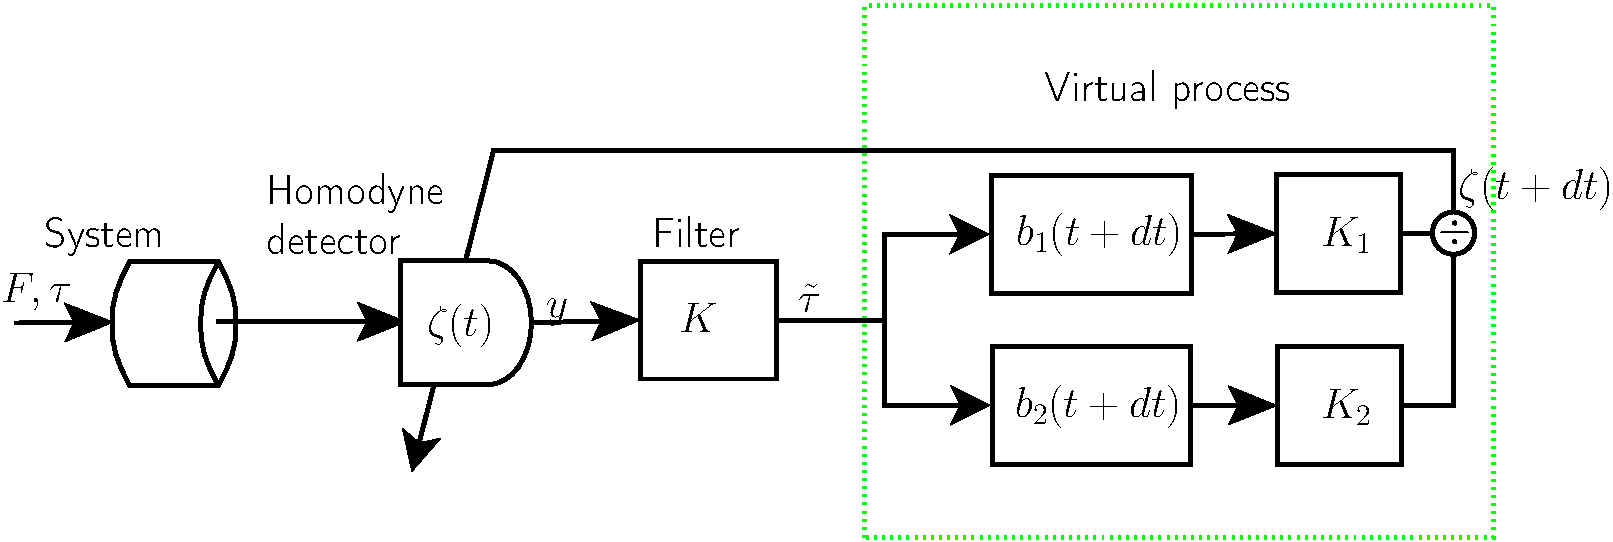
\includegraphics[width=0.95\textwidth]{process}}
\caption{Adaptive measurement scheme}
\label{pic:adaptive_process}
\end{figure}

The procedure of estimation is similar to described in previous section, but there are some significant differences.
Each time step we make two stage procedure (see Fig.\ref{pic:adaptive_process}):

\begin{enumerate}
 \item Estimation of arrival time.
  
On this stage we use all previous collected data for estimation the arrival time. At time $t$ we get some output from homodyne detector $y(t)$. Then we can use filter to get some estimation of arrival time $\tilde{\tau}$. This procedure is in some sense classical, because we use here only data that we have already collected for estimation the arrival time (the strict mathematical description we will provide below)
 \item Choice of optimal homodyne angle

In order to understand this stage we should turn to so-called variational measurements \cite{Vyatchanin1998m}. It uses correlation between measurement noise and back-action noise to evade the back-action. It can be shown mathematically (see Appendix \ref{appx:variational}) that in this case there's filtering function that lets us avoid the back-action.
The only restriction of this procedure is that we have to know arrival time. The same idea lyes in our procedure.

We use estimated arrival time to proceed back-action evading measurements. First we predict two quadratures $\hat{b}_{1,2}$ for next two time steps. We have to use two-steps because back-action affects on the system with time delay, so we can choose the optimal homodyne angle $\zeta(t+dt)$ for evading the back-action at time $t+2dt$. 
This procedure: prediction of quadratures, filtering and calculating the homodyne angle for the next step we do ``in our minds'' and we assume that it takes no time to do this, so it's like some virtual process (see Fig. \ref{pic:adaptive_virtual} )
\end{enumerate}
\begin{figure}
 \center{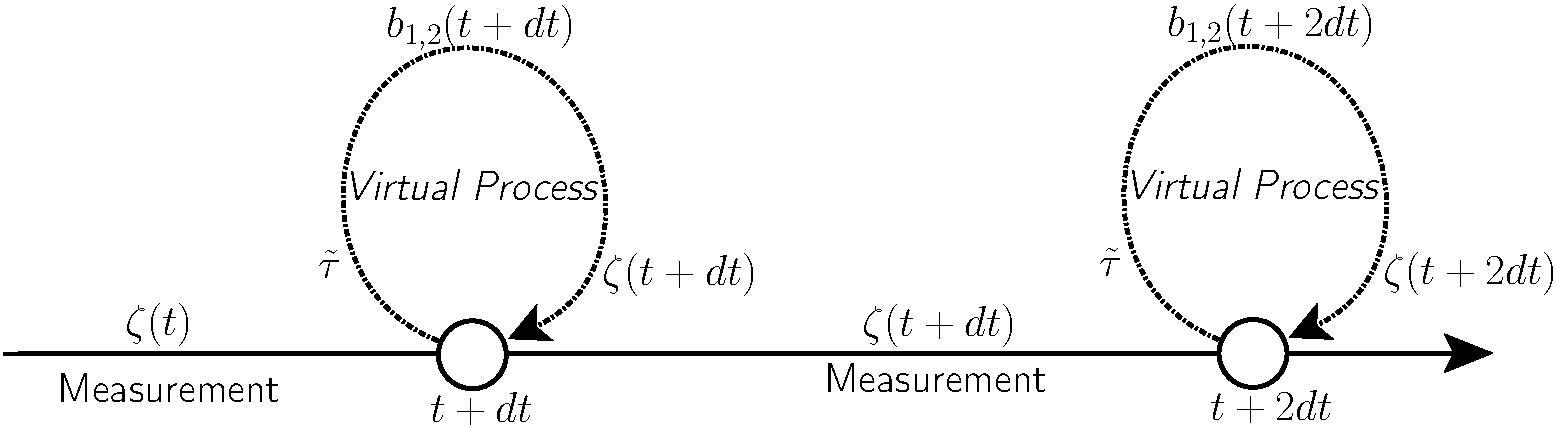
\includegraphics[width=0.9\textwidth]{process_sceme}}
\caption{Scheme for understanding the second stage.}
\label{pic:adaptive_virtual}
\end{figure}

This procedure can be described with a strict mathematics.
\subsubsection{First stage}
In our case we can write output as
\begin{equation}
 y(t)=\mathbb{C}(t)x+n(t)
\end{equation}
Here:
\begin{align}
& \mathbb{C}(t) = \sin\zeta(t)
\begin{bmatrix}
 \sin\omega_mt, & -\cos\omega_mt
\end{bmatrix}
\\
&
x=
\begin{bmatrix}
 A_c\\
A_s
\end{bmatrix}
\\
& n(t) = 
\begin{bmatrix}
 \cos\zeta(t), & \sin\zeta(t)
\end{bmatrix}
\begin{bmatrix}
 n_1(t)\\
n_2(t)
\end{bmatrix}
% =\mathbb{F}(t)\mathbb{N}(t)
\end{align}

We want to estimate two parameters $A_{c,s}$, using the filtering approach, as we mentioned before. In Appendix \ref{filtering} we show, how to get filtering function and derive estimation (see Eq.\ref{appx:est}):
\begin{equation}
 \tilde{x} =
\begin{bmatrix}
 \tilde{A_c}\\
\tilde{A_s}
\end{bmatrix}
= (\mathbb{D}^T\mathbb{N}^{-1}\mathbb{D})^{-1}\mathbb{D}^T\mathbb{N}^{-1}\mathbf{y}
\end{equation}

Here measurement matrix is
\begin{equation}
 \mathbb{D} = 
\begin{bmatrix}
 \mathbb{C}(t_0) \\
 \mathbb{C}(t_1) \\
 \vdots\\
 \mathbb{C}(t)
\end{bmatrix},
\end{equation}
signal vector is
\begin{equation}
 \mathbf{y} = 
\begin{bmatrix}
 y(t_0)\\
 y(t_1)\\
\vdots\\
y(t)
\end{bmatrix}
\end{equation}
and noise matrix is
\begin{equation}
 \mathbb{N} = 
\begin{bmatrix}
 \mean{n(t_0),n(t_0)} & \mean{n(t_0),n(t_1)} & \hdots & \mean{n(t_0),n(t)} \\
\mean{n(t_1),n(t_0)} & \mean{n(t_1),n(t_1)} & \hdots & \mean{n(t_1),n(t)} \\
\vdots & \vdots & \ddots & \vdots \\
\mean{n(t),n(t)} & \mean{n(t_1),n(t)} & \hdots & \mean{n(t),n(t)} \\
\end{bmatrix}
\end{equation}
where
\begin{equation}
 \mean{n(t_i)n(t_j)} = 
\begin{bmatrix}
 \cos\zeta(t), & \sin\zeta(t)
\end{bmatrix}
\begin{bmatrix}
 \mean{n_1(t_i),n_1(t_j)} & \mean{n_1(t_i),n_2(t_j)}\\
 \mean{n_2(t_i),n_1(t_j)} & \mean{n_2(t_i),n_2(t_j)}
\end{bmatrix}
\begin{bmatrix}
 \cos\zeta(t_j)\\ \sin\zeta(t_j)
\end{bmatrix}
\end{equation}

and

\begin{equation}\label{noises}
 \begin{cases}
  \means{\hat{n}_1(t)\hat{n}_1(t')}=&\frac{1}{2}\delta(t-t'),\\
  \means{\hat{n}_1(t)\hat{n}_2(t')}=&\frac{\alpha^2}{2\hbar}G(t'-t)\Theta(t'-t),\\
  \means{\hat{n}_2(t)\hat{n}_1(t')}=&\frac{\alpha^2}{2\hbar}G(t-t')\Theta(t-t'),\\
  \means{\hat{n}_2(t)\hat{n}_2(t')}=&\frac{1}{2}\delta(t-t')+\frac{\alpha^4}{4\hbar^2 m^2 \omega_m^2}\bigl(t'\cos\omega_m(t-t')-\frac{1}{\omega_m}\cos\omega_mt\sin\omega_mt'\bigr)\Theta(t-t')+\\
&+\frac{\alpha^4}{4\hbar^2 m^2 \omega_m^2}\bigl(t\cos\omega_m(t-t')-\frac{1}{\omega_m}\cos\omega_mt'\sin\omega_mt\bigr)\Theta(t'-t)+\\&+ \frac{\alpha^2}{2 m w \hbar}\cos\omega_m(t-t').
 \end{cases}
\end{equation}
% \begin{align}
% \bf{V}_1 =& 
%   \begin{bmatrix}
%   \begin{tabular}{cc|cccc}
%    $\mean{A_c, A_c}$ & $\mean{A_c, A_s}$&$\mean{A_c,y(t_1)}$ & $\mean{A_c,y(t_2)}$ & \ldots & $\mean{A_c,y(t)}$\\
%   $\mean{A_s, A_c}$ & $\mean{A_s, A_s}$&$\mean{A_s,y(t_1)}$ & $\mean{A_s,y(t_2)}$ & \ldots & $\mean{A_s,y(t)}$\\
%    \hline
%    $\mean{A_c, y(t_1)}$ & $\mean{A_s, y(t_1)}$ & $\mean{y(t_1),y(t_1)}$ & $\mean{y(t_1),y(t_2)}$ & \ldots & $\mean{y(t_1),y(t)}$\\ 
%   $\mean{A_c, y(t_2)}$ & $\mean{A_s, y(t_2)}$ & $\mean{y(t_2),y(t_1)}$ & $\mean{y(t_2),y(t_2)}$ & \ldots & $\mean{y(t_2),y(t)}$\\
%   $\vdots$ & $\vdots$ & $\vdots$ & $\vdots$ & $\ddots$ & $\vdots$\\
%  $\mean{A_c, y(t)}$ & $\mean{A_s, y(t)}$ & $\mean{y(t),y(t_1)}$ & $\mean{y(t),y(t_2)}$ & \ldots & $\mean{y(t),y(t)}$\\ 
% %   $\mean{x_0, b1(0)}$ & $\mean{b_1(0),b_1(0)}$ & $\mean{b_1(0),b_2(0)}$ & \ldots & $\mean{b_1(t+dt),b_1(t+dt)}$ & $\mean{b_1(t+dt),b_2(t+dt)}$\\ 
% % $\mean{x_0, b2(0)}$ & $\mean{b_2(0),b_1(0)}$ & $\mean{b_2(0),b_2(0)}$ & \ldots & $\mean{b_2(t+dt),b_1(t+dt)}$ & $\mean{b_2(t+dt),b_2(t+dt)}$\\ 
% %  
%   \end{tabular}
%  \end{bmatrix}
% =\\=&
% \begin{bmatrix}
%   \begin{tabular}{c|c}
%   $V_{xx}^{(1)}$ & $V_{xy}^{(1)}$\\
%   \hline
%   ${V_{xy}^{(1)}}^T$ & $V_{yy}^{(1)}$
%  \end{tabular}
%  \end{bmatrix}
% \end{align}

% Then we calculate estimation for vector 
% \begin{equation}
%   \tilde{\mathbb{X}} = 
%  \begin{bmatrix}
%   \tilde{A}_c \\ \tilde{A}_s
%  \end{bmatrix}
% = V_{xy}^{(1)}{V_{yy}^{(1)}}^{-1}y
% \end{equation}
Using this estimation,we get the estimated arrival time:
\begin{equation}
 \tilde{\tau} = \frac{1}{\omega_m}\arctan \frac{\tilde{A}_s}{\tilde{A}_c}
\end{equation}
This equation describes the estimation for arrival time that we get on each time step.

\subsubsection{Second stage}
In previous step we used the knowledge about measurement results in the past. Now we want to make prediction about next measurement in order to find optimal homodyne angle.
Suppose, that we can make prediction about both quadratures $b_{1,2}$. Then:
\begin{equation}
 \begin{cases}\label{b1b2}
  \hat{b}_1(t) = \hat{a}_1(t) \\
  \hat{b}_2(t) = \hat{a}_2(t)+ I(t) + \frac{\alpha^2}{\hbar}\int\limits_0^{\infty} dt' \, G(t-t') \,\Theta(t-t') \hat{a}(t') + \frac{\alpha}{\hbar}x_0 \sin \omega_m (t-\tilde{\tau})
 \end{cases}
\end{equation}
In back-action term we can use sum instead of the integral. So we can write this integral as product of two vectors:
\begin{equation}
 \I{0}{t}d\tau\, G(t-\tau)a_1(\tau) = \lim\limits_{dt\rightarrow0}\sum\limits_{i=1}^NG(t-t_i) a_1(t_i) dt = \lim\limits_{dt\rightarrow0} 
\begin{bmatrix}
 G(t-t_1), & G(t-t_2), & \hdots, & G(t-t_N)
\end{bmatrix}
\begin{bmatrix}
 a_1(t_1)\\a_1(t_2)\\\vdots\\a_2(t_N)
\end{bmatrix}
dt
\end{equation}
where $t_i = i\,dt, t_N = t$
For any moment of time $t$ we can compute back-action matrix as:
\begin{equation}
 \begin{bmatrix}
  BA(t_1)\\BA(t_2)\\\vdots\\BA(t)
 \end{bmatrix}
=\alpha
\begin{bmatrix}
 0 & 0 & 0 &\hdots & 0\\
 G(t_2-t_1) &0 &0 &\hdots & 0\\
 G(t_3-t_1) &G(t_3-t_2) &0 &\hdots & 0\\
\vdots &\vdots &\vdots &\ddots & \vdots\\
G(t-t_1) &G(t-t_2) &G(t-t_3) &\hdots & 0
\end{bmatrix}
\begin{bmatrix}
 a_1(t_1)\\a_1(t_2)\\\vdots\\a_2(t)
\end{bmatrix}
dt
\end{equation}

Here we can use the same filtering approach, but now for two quadratures:
\begin{equation}
 \begin{bmatrix}
  \hat{b}_1(t+dt)\\ \hat{b}_2(t+dt)
 \end{bmatrix}
=
\begin{bmatrix}
 0 \\ \frac{\alpha}{\hbar} \sin \omega_m(t+dt)
\end{bmatrix}
x_0 + I(t)+
\begin{bmatrix}
 \hat{n}_1(t+dt) \\ \hat{n}_2(t+dt)
\end{bmatrix}
\end{equation}

Then covariation matrix between signal and output would be:
{\tiny
\begin{equation}
\hspace{-2cm} \bf{V}_2 = 
 \begin{bmatrix}
 \begin{tabular}{c|c|cccc}
   $\mean{x_0, x_0}$ & $V_{xy}^{(1)}$ & $\mean{x_0,b_1(t+dt)}$ & $\mean{x_0,b_2(t+dt)}$ & $\mean{x_0,b_1(t+2dt)}$ & $\mean{x_0,b_2(t+2dt)}$\\
   \hline
   ${V_{xy}^{(1)}}^T$  & $V_{yy}^{(1)}$ & 
$\begin{matrix}
\mean{y(t_1),b_1(t+dt)}\\
\vdots \\
\mean{y(t),b_1(t+dt)} \\
\end{matrix}$ & $\begin{matrix}
\mean{y(t_1),b_2(t+dt)}\\
\vdots\\
\mean{y(t),b_2(t+dt)}\\
\end{matrix}$ &
$\begin{matrix}
\mean{y(t_1),b_1(t+2dt)}\\
\vdots \\
\mean{y(t),b_1(t+2dt)} \\
\end{matrix}$ & $\begin{matrix}
\mean{y(t_1),b_2(t+2dt)}\\
\vdots\\
\mean{y(t),b_2(t+2dt)}\\
\end{matrix}$\\
\hline
$\mean{b_1(t+dt),x_0}$ & 
$\begin{matrix}
\mean{b_1(t+dt),y(t_1)} & \ldots & \mean{b_1(t+dt),y(t)} \\
\end{matrix}$ & $\mean{b_1(t+dt),b_1(t+dt)}$ & $\mean{b_1(t+dt),b_2(t+dt)}$ & $\mean{b_1(t+dt),b_1(t+2dt)}$ & $\mean{b_1(t+dt),b_2(t+2dt)}$\\
$\mean{b_2(t+dt),x_0}$ & 
$\begin{matrix}
\mean{b_2(t+dt),y(t_1)} & \ldots & \mean{b_2(t+dt),y(t)} \\
\end{matrix}$ & $\mean{b_2(t+dt),b_1(t+dt)}$ & $\mean{b_2(t+dt),b_2(t+dt)}$& $\mean{b_2(t+dt),b_1(t+2dt)}$ & $\mean{b_2(t+dt),b_2(t+2dt)}$\\
$\mean{b_1(t+2dt),x_0}$ & 
$\begin{matrix}
\mean{b_1(t+2dt),y(t_1)} & \ldots & \mean{b_1(t+2dt),y(t)} \\
\end{matrix}$ & $\mean{b_1(t+2dt),b_1(t+dt)}$ & $\mean{b_1(t+2dt),b_2(t+dt)}$ & $\mean{b_1(t+2dt),b_1(t+2dt)}$ & $\mean{b_1(t+2dt),b_2(t+2dt)}$\\
$\mean{b_2(t+2dt),x_0}$ & 
$\begin{matrix}
\mean{b_2(t+2dt),y(t_1)} & \ldots & \mean{b_2(t+2dt),y(t)} \\
\end{matrix}$ & $\mean{b_2(t+2dt),b_1(t+dt)}$ & $\mean{b_2(t+2dt),b_2(t+dt)}$ & $\mean{b_2(t+2dt),b_1(t+2dt)}$ & $\mean{b_2(t+2dt),b_2(t+2dt)}$
  \end{tabular}
 \end{bmatrix}
\end{equation}
}
Then filter is
\begin{equation}
\mathbb{K}_2 = V_{xy}^{(2)}{V_{yy}^{(2)}}^{-1} = 
\begin{bmatrix}
 K_{y(t_1)}\\K_{y(t_2)}\\\vdots\\K_{y(t)} \\K_1(t+dt)\\K_2(t+dt)\\K_1(t+2dt)\\K_2(t+2dt)
\end{bmatrix}
\end{equation}
where 
\begin{equation}
  V_{xy}^{(2)} = 
\begin{bmatrix}
 V_{xy}^{(1)}, & \mean{x_0,b_1(t+dt)}, & \mean{x_0,b_2(t+dt)} & \mean{x_0,b_1(t+2dt)}, & \mean{x_0,b_2(t+2dt)}
\end{bmatrix}
\end{equation}
Here we remember that we have to get homodyne angle at time $t+dt$ to evade the back-action at time $t+2dt$
Then due to the fact that readout is $$Y(t+dt)=K_1(t+dt) b_1(t+dt) + K_2(t+dt) b_2(t+dt) = g \cos\zeta(t+dt)b_1(t+dt)+g\sin\zeta(t+dt)b_2(t+dt)$$ 
we can find homodyne angle as
\begin{equation}
 \zeta(t+dt) = \arctan\frac{K_2(t+dt)}{K_1(t+dt)}
\end{equation}

If we compute all the covariation functions, we get:
\begin{equation}
 \means{x_0,x_0} = \sigma_{x_0}
\end{equation}
\begin{align}
& \means{x_0,b_1(t+dt)} = 0\\
& \means{x_0,b_2(t+dt)} = \frac{\alpha}{\hbar}\sigma_{x_0} \sin\omega_m(t+dt-\tilde{\tau})
\end{align}

And output correlations with signal at time $t_j<t_i$:
\begin{equation}
\begin{cases}
\means{b_1(t_i),y(t_j)} = 0\\
\means{b_2(t_i), y(t_j)} = \means{b_2(t_i),b_1(t_j)}\cos\zeta(t_j) + \means{b_2(t_i),b_2(t_j)}\sin\zeta(t_j)
\end{cases}
\end{equation}
 \section{Results}
For presenting some numerical result we wrote a program that simulates working cycle of the adaptive algorithm.
Our algorithm rotates homodyne angle for getting the best estimation by means of cancelling the back action. On Fig. \ref{alpha_10} (left) we can see, how homodyne angle depends on time.
\begin{figure}[t]
 \begin{minipage}{0.5\linewidth}
  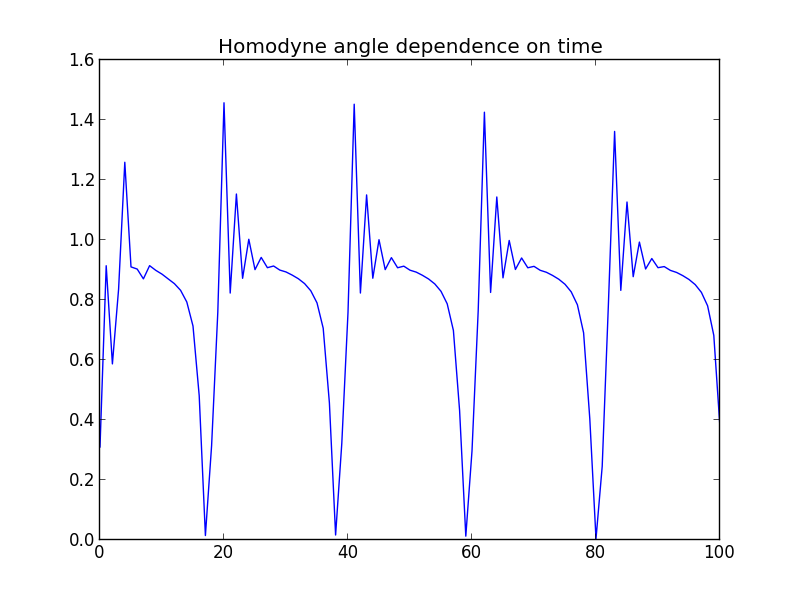
\includegraphics[width=1.\linewidth]{z_big_F}
 \end{minipage}
\hfill
 \begin{minipage}{0.5\linewidth}
  \center{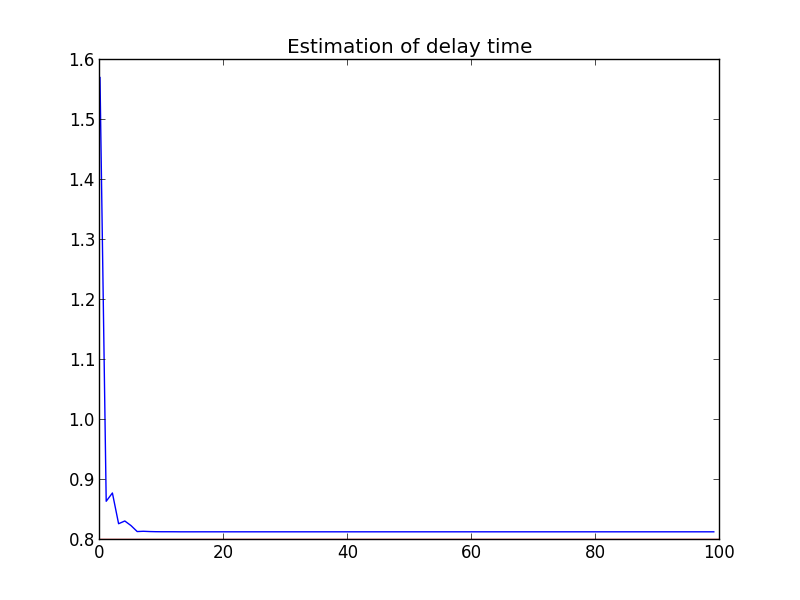
\includegraphics[width=1.\linewidth]{T_a10_big}}
 \end{minipage}
\caption{Homodyne angle $\zeta(t)$ dependence on time \textit{(left)} and estimation of delay time depending on time \textit{(right)}.}
\label{alpha_10}
 \end{figure}
Also we can see how our algorithm estimates the arrival time (See  Fig. \ref{alpha_10} (right)). Then for compartment we place how estimation algorithm works in adaptive measurements and in measurements with fixed homodyne angle (see Fig.\ref{FbAb}).
\begin{figure}[h]
 \begin{minipage}{0.5\textwidth}
  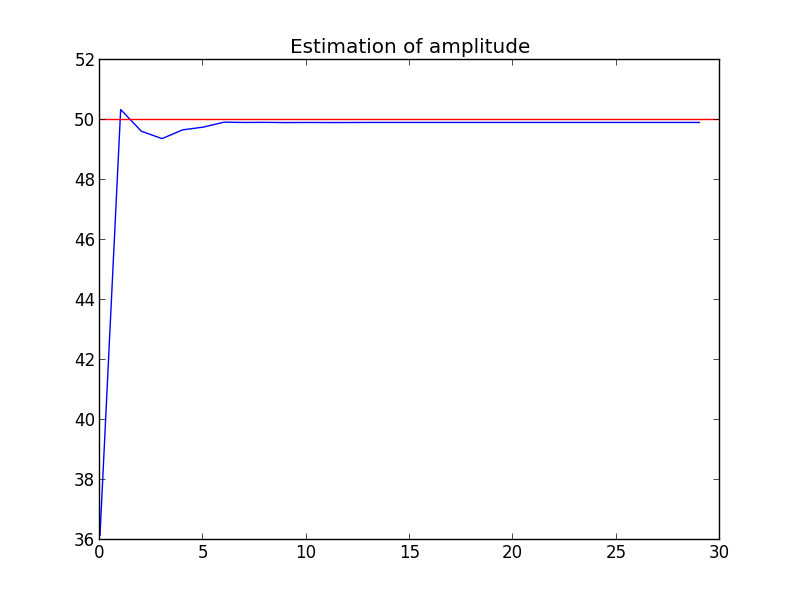
\includegraphics[width=1.\linewidth]{F_a10_big}
 \end{minipage}
\hfill
 \begin{minipage}{0.5\textwidth}
  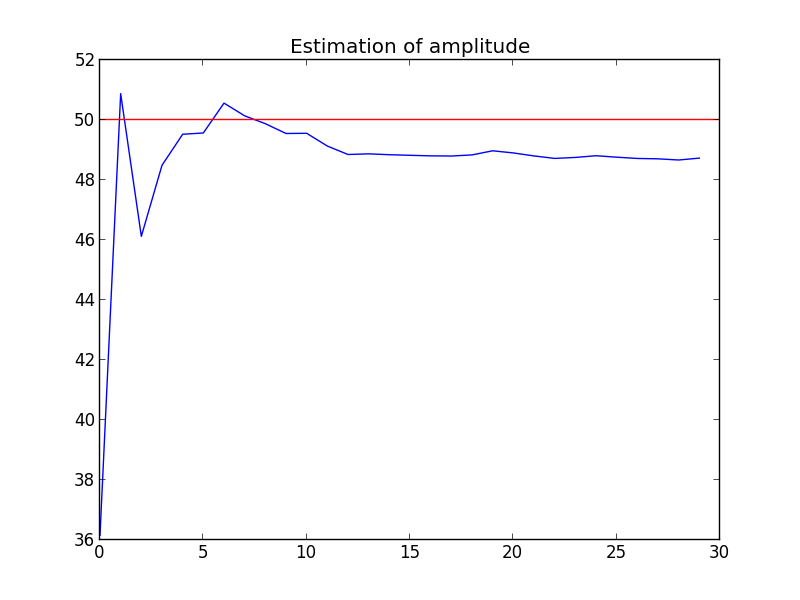
\includegraphics[width=1.\linewidth]{F_a10_big_ph}
 \end{minipage}
\caption{Compare the estimation of amplitude in adaptive measurements\textit(left) and measurements with fixed homodyne angle \textit{right}}
\label{FbAb}
\end{figure}
Finally we place here some numerical results (see Table \ref{set1}). All the results we discuss in the next section.
\begin{table}[h!]
 \center{\begin{tabular}{|c||c|c|c|c|}
  \hline
    & $\bar{F}_{est}$ & $\Delta F$ &  $\bar{\tau}_{est}$ & $\Delta \tau$\\
\hline
 Variational readout & -- & 0.0015 &  -- & -- \\
\hline
Adaptive measurement & 51.122 & 0.022 & 0.9 & 0.0004 \\
\hline
Fixed homodyne angle $\zeta = \pi/2$  & 51.035 & 0.064 & 0.9023 & 0.0023 \\
\hline
 \end{tabular}}
\caption{$\tau = 0.9, F = 51.1, N = 1000,T=6.6$}
\label{set1}
\end{table}
\include{conversation}
%------------------------------------------------------------------------------------------------------
\newpage
\appendix
\section{Conservation of optimal estimation while mapping}\label{Appendix 1}
If the estimation is optimal it means that dispersion is minimal and then we can say that von Neumann entropy is maximal:
\begin{align}
& S = -\Tr{\rho(x) \ln \rho(x)}, \\
& \delta S = 0, \\
& \delta^2 S <0,
\end{align}
where $\rho(x)$ is density matrix that depends on parameter vector $x = \{x_1,x_2,...,x_n\}$.

Then we can write for other coordinates $y=y(x)$
\begin{equation}
 \delta S = dS = \sum\limits_{i=1}^n \frac{\partial S}{\partial \rho(x_i)}d\rho(x_i)=\sum\limits_{i=1}^n \frac{\partial S}{\partial \rho(x_i)}\frac{d \rho(x_i)}{d x_i}dx_i =\sum\limits_{i=1}^n \frac{\partial S}{\partial \rho(y_i)}\frac{d \rho(y_i)}{d y_i}\frac{d y_i}{d x_i}dx_i =0
\end{equation}
Then 
\begin{equation}\label{app:zero}
\frac{\partial S}{\partial \rho(x_i)} = \frac{\partial S}{\partial \rho(y_i)} = 0
\end{equation}
if $\frac{\rho(y_i)}{\rho(x_i)}\neq0$. So, if $dS(x)=0$ then $dS(y)=0$
And, for the second derivative:
\begin{equation}\label{app:d2}
 \delta^2 S = d^2 S(x) = \sum\limits_{i,j=1}^n \frac{\partial^2 S}{\partial \rho(x_i) \partial \rho(x_j)}d\rho(x_i)d\rho(x_j)
\end{equation}
This equation can be simplified using Eq.\ref{app:zero}: all the mixed therms would be equal to zero.
Then we get from Eq.\ref{app:d2}:
\begin{equation}
 d^2 S(x) = \sum\limits_{i=1}^n \frac{\partial^2 S}{\partial \rho(x_i)^2 }(d\rho(x_i))^2<0
\end{equation}
Because of the positive definition of $(d\rho(x_i))^2$ we can write, that $\frac{\partial^2 S}{\partial \rho(x_i)^2 } < 0$ and for other coordinates:
\begin{equation}
 d^2 S(y) = \sum\limits_{i=1}^n \frac{\partial^2 S}{\partial \rho(y_i)^2 }(d\rho(y_i))^2 = \sum\limits_{i=1}^n \frac{\partial^2 S}{\partial \rho(x_i)^2 }(d\rho(x_i))^2 <0
\end{equation}

We proved that for any change of coordinates the maximum of entropy conserves and then conserves the optimum of the estimation.
\section{Linear estimation\cite{S.N1993}}\label{filtering}
Consider output signal to be
\begin{equation}
  \mathbf{y} = \mathbb{D} x + \mathbf{n},
\end{equation}
where $\mathbf{y}$ is a $N\times1$ vector, $\mathbb{D}$ is a known $N\times p$ matrix, $x$ is a $p\times 1$ vector of parameters, $\mathbf{n}$ is a 
$N\times1$ noise vector with zero mean and covariance $\mathbb{N}$.

We want to get unbiased estimation of $x$, assuming no prior knowledge about this signal. This estimation would be:
\begin{equation}
 x = \mathbb{L}\mathbf{y},
\end{equation}
where $\mathbb{L}$ is filtering function.

The condition of unbiasedness leads to the following:
\begin{equation}
 E[\hat{x}] = \mathbb{L} E[\mathbf{y}] = x
\end{equation}
and noticing the zero mean of the noise:
\begin{equation}
 E[\mathbf{y}] = \mathbb{D} x,
\end{equation}
then we get the constraint for filtering function:
\begin{equation}\label{appx:constraint}
 \mathbb{L}\mathbb{D} = \mathbb{I}.
\end{equation}
Our aim is to find optimal in sense of minimal of variation filtering function.
Variation of the estimation is:
\begin{equation}\label{appx:var}
 var(\hat{x}) = E[(x-\hat{x})^2] = E[(\mathbb{L}(E[\mathbf{y}] - \mathbf{y}))^2] = E[\mathbb{L}(\mathbf{y}-E[\mathbf{y}])(\mathbf{y}-E[\mathbf{y}])^T\mathbb{L}^T] =\mathbb{L}\mathbb{N}\mathbb{L}^T 
\end{equation}
We should take into account the constraint\label{appx:constraint} and construct Lagrange function:
\begin{equation}
 J[\mathbb{L}] = \mathbb{L}\mathbb{N}\mathbb{L}^T + \lambda (\mathbb{L}\mathbb{D} - \mathbb{I})
\end{equation} 
Then we calculate functional derivative over filtering function:
\begin{equation}
 \delta J[\mathbb{L}] = \delta \mathbb{L} \bigl(2 \mathbb{N}\mathbb{L}^T + \mathbb{D}\lambda \bigr) = 0
\end{equation}
Then 
\begin{equation}
 \mathbb{L}^T = -\frac{1}{2}\mathbb{N}^{-1}\mathbb{D}\lambda
\end{equation}
and 
\begin{equation}
 \mathbb{D}^T\mathbb{L}^T =  -\frac{1}{2}\mathbb{D}^T\mathbb{N}^{-1}\mathbb{D}\lambda = \mathbb{I},
\end{equation}
So we get an equation for $\lambda$:
\begin{equation}
 -\frac{1}{2}\lambda = (\mathbb{D}^T\mathbb{N}^{-1}\mathbb{D})^{-1},
\end{equation}
\begin{equation}
 \mathbb{L}^T = \mathbb{N}^{-1}\mathbb{D}(\mathbb{D}^T\mathbb{N}^{-1}\mathbb{D})^{-1}
\end{equation}
and finally we get an equation for filtering function:
\begin{equation}\label{appx:est}
 \mathbb{L} = (\mathbb{D}^T\mathbb{N}^{-1}\mathbb{D})^{-1}\mathbb{D}^T\mathbb{N}^{-1}
\end{equation}
We can also simply calculate the variation for this estimation (see Eq.\ref{appx:var}).
\begin{equation}
 \tilde{x} = \mathbb{L}\mathbb{N}\mathbb{L}^T = (\mathbb{D}^T\mathbb{N}^{-1}\mathbb{D})^{-1}\mathbb{D}^T\mathbb{N}^{-1}\mathbb{N}\mathbb{N}^{-1}\mathbb{D}(\mathbb{D}^T\mathbb{N}^{-1}\mathbb{D})^{-1} = (\mathbb{D}^T\mathbb{N}^{-1}\mathbb{D})^{-1}
\end{equation}


\section{Variational measurements}\label{appx:variational}

Let's derive how homodyne angle changes in time.

The output signal would be:
\begin{multline}
 y(t)=\hat{b}_1(t)\cos\zeta(t)+\hat{b}_2(t)\sin\zeta(t) = \\
=\hat{a}_1(t)\cos \zeta(t)+\Bigl[\hat{a}_2(t)+\frac{\alpha}{\hbar}\bigl(\alpha \int\limits_0^{T} dt' \, G(t-t') \, \hat{a}(t') + \frac{\bar{F}}{m\omega_m}\sin\omega_m(t-\tau)\bigr)\Bigr]\sin\zeta(t)
\end{multline}

And after filtering with filtering function $g(t)$:
\begin{equation}
 Y=\I{0}{T}dt'\,(g(t')\hat{b}_1(t')\cos\zeta(t')+g(t')\hat{b}_2(t')\sin\zeta(t')) = \I{0}{T}dt'(g_1(t')\hat{b}_1(t')+g_2(t')\hat{b}_2),
\end{equation}
where $g_1(t)=g(t)\cos\zeta(t), g_2(t)=g(t)\sin\zeta(t)$.
Or, we can write:
\begin{equation}
 Y = \I{0}{T} dt' \bigl(g_1(t')a_1(t')+g_2(t')\frac{\alpha^2}{\hbar}\I{0}{\infty}dt''G(t'-t'')\Theta(t'-t'')a_1(t'') + g_2(t')a_2(t')\bigr) + \frac{\alpha}{\hbar}\I{0}{T}dt'\,g_2(t')x_0\sin\omega_m(t'-\tau)
\end{equation}
Then, after changing the oder of interals, we can write down the equation for back-action evaison:
\begin{equation}\label{BAE}
 g_1(t)+\frac{\alpha^2}{\hbar}\I{t}{T}dt'\,g_2(t')G(t'-t)=0
\end{equation}
and then for $Y$ we get:
\begin{equation}
 Y_{BAE} = \I{0}{T} dt' \bigl(g_2(t')a_2(t') + \frac{\alpha}{\hbar}g_2(t')x_0\sin\omega_m(t'-\tau)\bigr)
\end{equation}
We can assume for maximizing the signal,that we have constraint:
\begin{equation}
 \frac{\alpha}{\hbar}\I{0}{T}dt'\,g_2(t')\sin\omega_m(t'-\tau) = 1
\end{equation}
Then we construct Lagrangian function:
\begin{equation}\label{L}
 \mathcal{L}[g_2(t)] = \mean{Y^2} + \mu (\frac{\alpha}{\hbar}\I{0}{T}dt'\,g_2(t')\sin\omega_m(t'-\tau) - 1)
\end{equation}
Here 
\begin{equation}\label{<Y>}
 \mean{Y^2} = \frac{1}{2}\I{0}{T}dt'g_2^2(t') + x_0^2
\end{equation}
because $\mean{a_2(t)a_2(t')}=\frac{1}{2}\delta(t-t')$.
Then from Eq.\ref{L} we can calculate the variation of Lagrangian:
\begin{equation}
 \delta\mathcal{L}[g_2(t)] = \frac{1}{2}\delta\I{0}{T}dt'g_2^2(t') + \mu \delta(\frac{\alpha}{\hbar}\I{0}{T}dt'\,g_2(t')\sin\omega_m(t'-\tau) - 1)
\end{equation}
After calculation the variation:
\begin{equation}
 \delta\mathcal{L}[g_2(t)] = \I{0}{T}dt'\delta g_2(t')(g_2(t') + \mu \frac{\alpha}{\hbar}\sin\omega_m(t'-\tau)) = 0
\end{equation}
or, as to the fact that $\delta g_2(t') \neq 0$
\begin{equation}
\begin{cases}
 g_2(t) + \mu \frac{\alpha}{\hbar}\sin\omega_m(t-\tau) = 0\\
\frac{\alpha}{\hbar}\I{0}{T}dt'\,g_2(t')\sin\omega_m(t'-\tau) = 1
\end{cases}
\end{equation}
Solving this system of equations, we get:
\begin{equation}\label{g2}
 g_2(t) = \frac{4\omega_m\hbar}{\alpha} \frac{\sin\omega_m(t-\tau)}{2\omega_mT-\sin2\omega_m(T-\tau)-\sin2\omega_m\tau}
\end{equation}
Then we can substitute Eq.\ref{g2} to Eq.\ref{BAE} and get equation for $g_1(t)$
\begin{equation}\label{g1}
 g_1(t) = \frac{\alpha}{m \omega_m} \frac{-2\omega_m(t-T)\cos\omega_m(t-\tau) + \sin\omega_m(t-\tau) + \sin\omega_m(t-2T+\tau)}{-2T\omega_m + \sin2\omega_m(T-\tau)+\sin2\omega_m\tau}
\end{equation}
So,we can get analytical equation for homodyne angle from Eq.\ref{g1},\ref{g2}:
\begin{equation}\label{appx:zeta}
 \zeta(t) = \arctan\frac{g_2(t)}{g_1(t)}
\end{equation}

Finally an error in estimation the force would be (see Eq.\ref{<Y>} and \ref{g2})
\begin{equation}
 \Delta F = \frac{2\omega_m\hbar^2}{\alpha^2} \frac{1}{2\omega_mT-\sin2\omega_m(T-\tau)-\sin2\omega_m\tau}
\end{equation}

\newpage
\bibliography{Bibtex/adaptive,Bibtex/mqm,Bibtex/mqm_my,Bibtex/ligo,Bibtex/ligo_my,Bibtex/biblio_u,Bibtex/misc_u}

\end{document}